%Introduction Pragraph

%How did you generate your preliminary design ideas? Why do you choose the current design. Do you have some other preliminary designs that can be compared with to show the superiority of your current design?

To generate our preliminary design, we simply thought of an initial idea, implicated a change to the initial design that we thought was feasibly possible. Then, with some modifications, we came across the first roadblock of accurately sizing every individual piece so that they could mesh together to create a functioning body. We used the insight to first create our own individual parts to the specific sizes we intended, and then during the assembly phase of the project, we encountered the struggle of the differing sizes in our own vision, which in turn caused heavy modifications for the drone to not only function but to even be plausible. After various trials during assembly, we came across our final design, which we stuck through till the end so we could make the best and most functioning drone we could come up with. 

\subsection{Product Specifications}
% Give a full introduction of your design

Our design as seen in Figure 3-1 has taken inspiration after DOR-15. Our drone takes the shape of a bowler hat, which takes a turn from traditional drone designs. While this may not be the typical drone that people expect to see, we think that our hat can exceed people's expectation. The toy of tomorrow is here today, to be every child's newest companion and every parent's handy helper.

\subsection{Details of the Design}
%Include a picture of the entire assembled model here. Explain your design. All other CAD models should be placed in the appropriate appendix.

Starting at the exterior of DORIS, it utilities three propellers to move around in 6 degrees of freedom. The front side of DORIS has the option to install a camera module to further help with navigation and assisting in tasks its owner may designate. These propellers are connected with a dowel that extends into the hat. For future models, we place to shorten these dowels or make them retractable in order for the user to wear the hat also. Currently, to prevent the user from using the hat in flight mode, we have installed a parts cover on the bottom to prevent dust and damage to the dowels and propellers. On the inside of the hat would be where the brain/computer of DORIS would lay and control all decision making and navigation. This is not indicated on the model but would be useful for future iterations.

    \begin{figure}
        \centering
        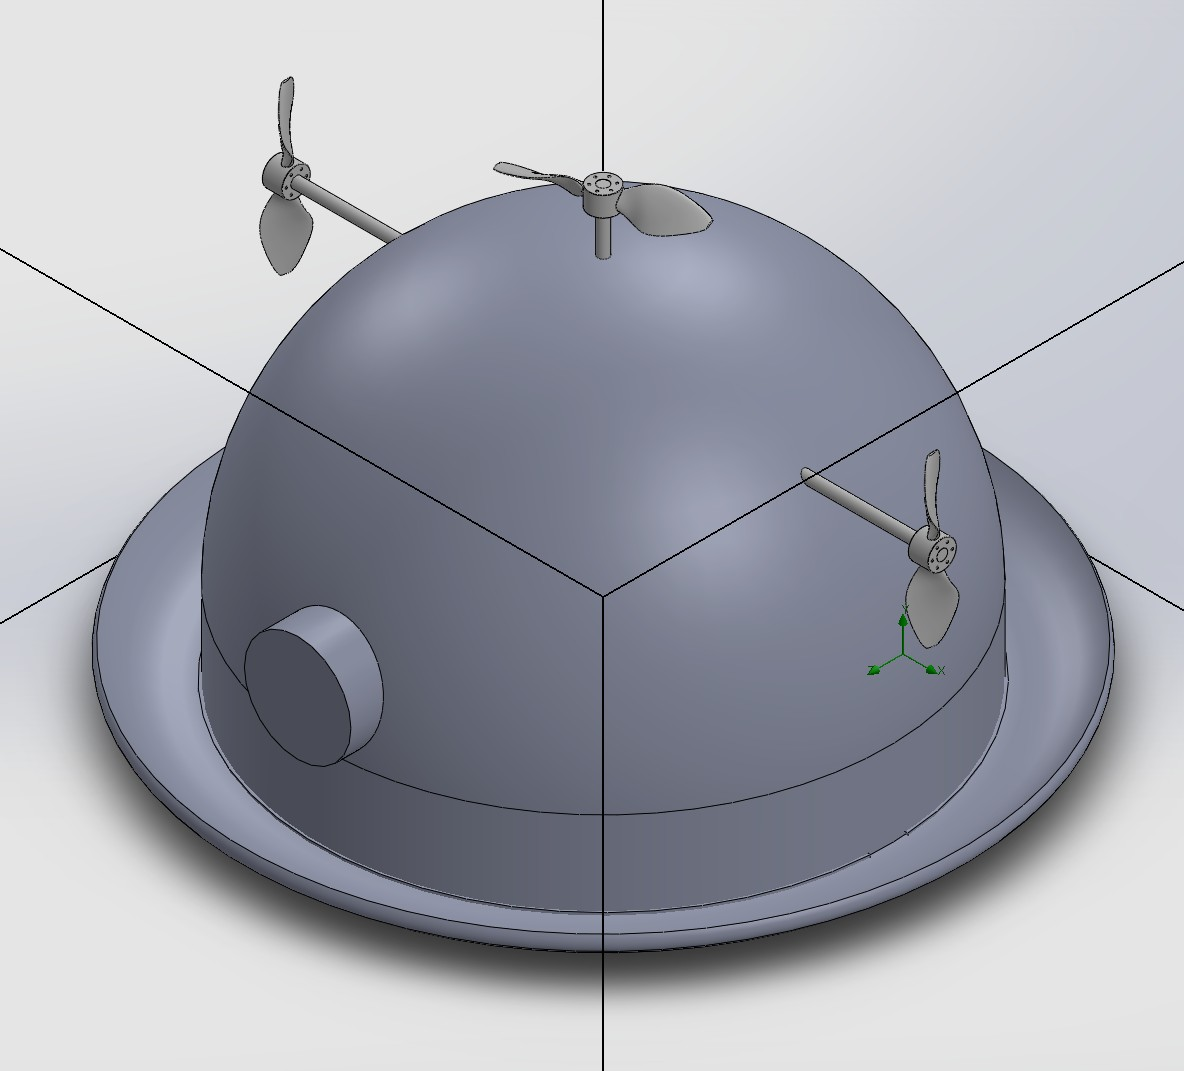
\includegraphics[width=0.5\linewidth]{root/Models/Hat_Model.jpg}
        \caption{Isometric View of the Final Assembly}
        \label{fig:Hat Assembly}
    \end{figure}


\subsection{Tolerance and Fit}
%Point out the tolerance and fit of the connecting parts. You should give reasonable tolerance for the parts and fit for the connections. At the same time give an explanation of why. Show tolerance and fit in the CAD drawing. Explain everything in your Presentation


In terms of fits, our drone was given a small bit of leeway. Our dowels were force fit in the center of the propeller in order to ensure the propeller would not fall off. There is a tolerance on the dowel in order to make sure it supports the weight of the propeller. The parts cover also received a small tolerance in order to ensure manufacturing this part would fit all hats without forgoing quality.